\documentclass[11pt]{article}

%Don't change any thing before \begin{document}
%In fact if you use sth fancy, you might need
%to add more packages, or macros.

\usepackage{times,psfrag,epsf,epsfig,graphics}


\usepackage{../EllioStyle}



\begin{document}
\date{Feb 18, 2020}
\ShortHeadings{Computer Science Theory: Assignment~1}{Elliott Pryor}
\title{CSCI 338: Assignment~2~(6 points)}

\author{Elliott Pryor}


\maketitle

%When writing up your solution, comment out the following until you reach Problem 1.
\noindent
This assignment is due on {\bf Tuesday, Feb 18, 11:30pm}. It is strongly
encouraged that you use Latex to generate a single pdf file and upload it
under {\em Assignment 2} on D2L. But there will NOT be a penalty for not
using Latex (to finish the assignment). This is {\bf not} a group-assignment,
so you must finish the assignment by yourself.

\newpage
\section*{Problem 1}

\noindent
(1.1) Problem 1.6.c, 1.6.f (page 84---
all the questions with only numbers given are referred to the 3rd edition of the textbook).
\newline

\textbf{1.6.c}

 \begin{figure}[H]
     \centering
     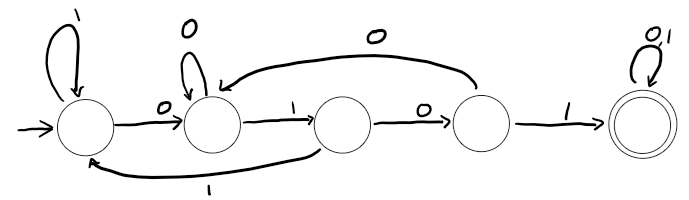
\includegraphics[width = 0.8\textwidth]{16c_CSCI338.PNG}
     \caption{Solution to 1.6.c}
     \label{fig:1.6.c}
 \end{figure}
 
\textbf{1.6.f}
  \begin{figure}[H]
     \centering
     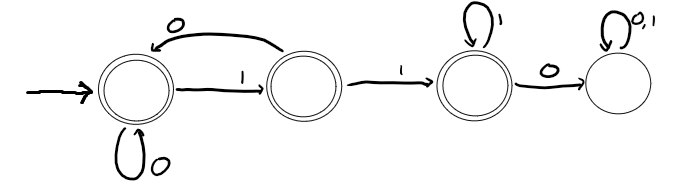
\includegraphics[width = 0.8\textwidth]{16f_CSCI338.PNG}
     \caption{Solution to 1.6.f}
     \label{fig:1.6.f}
 \end{figure}

\noindent
(1.2) Problem 1.7.b, 1.7.c (page 84).
\newline

\textbf{1.7.b}

The solution for 1.6.c (Figure \ref{fig:1.6.c}) is also a valid NFA and has 5 states.

\textbf{1.7.c}
  \begin{figure}[H]
     \centering
     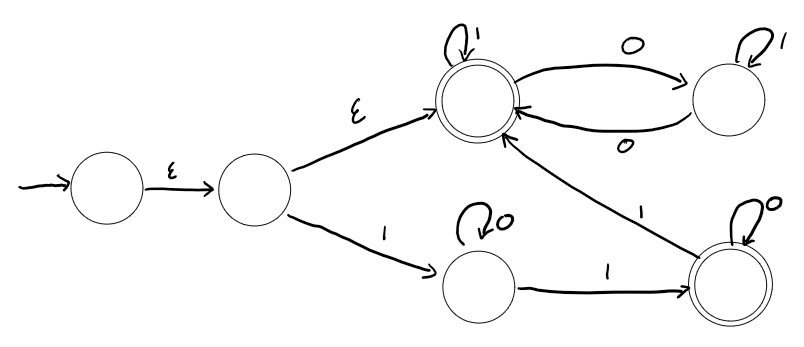
\includegraphics[width = 0.84\textwidth]{17c_CSCI338.PNG}
     \caption{Solution to 1.7.c}
     \label{fig:1.7.c}
 \end{figure}


\newpage
\section*{Problem 2}

Problem 1.16.a, ~Problem 1.16.b (page 86).
\newline

\textbf{1.16.a}
\begin{figure}[H]
     \centering
     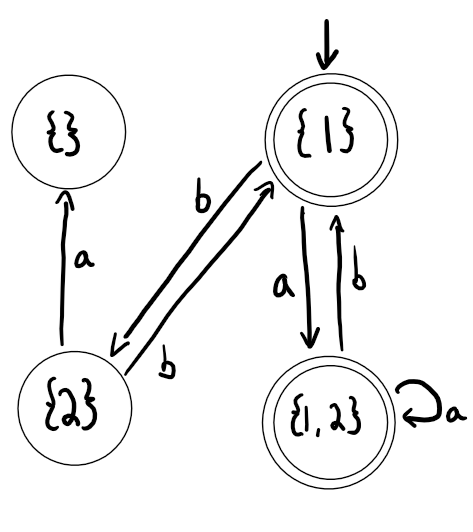
\includegraphics[width = 0.5\textwidth]{1_16a_CSCI338.PNG}
     \caption{Solution to 1.16.a}
     \label{fig:1.16.a}
 \end{figure}  
 
 
\textbf{1.16.b}
\begin{figure}[H]
     \centering
     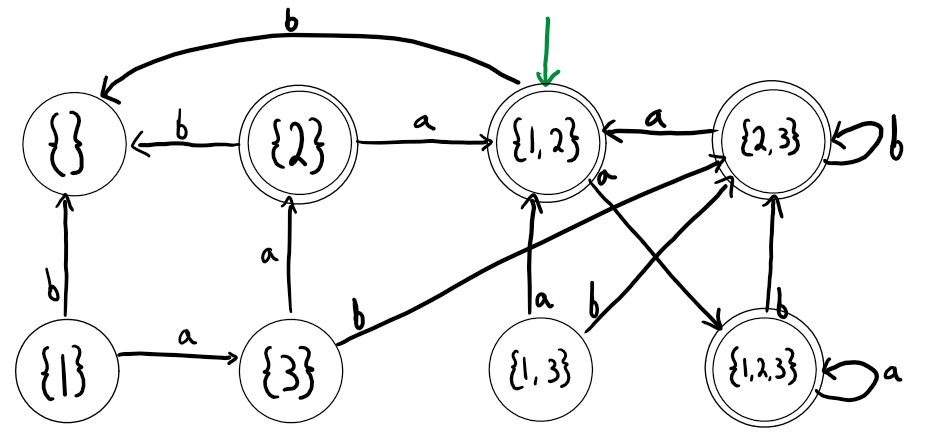
\includegraphics[width = 0.8\textwidth]{1_16b_CSCI338.PNG}
     \caption{Solution to 1.16.b}
     \label{fig:1.16.b}
 \end{figure}



\newpage
\section*{Problem 3}

Problem 1.19.a, 1.19.b (page 86).
\newline

Note in solutions some of the internal epsilon transitions are ommitted for concision. 

\textbf{1.19.a}

\begin{figure}[H]
     \centering
     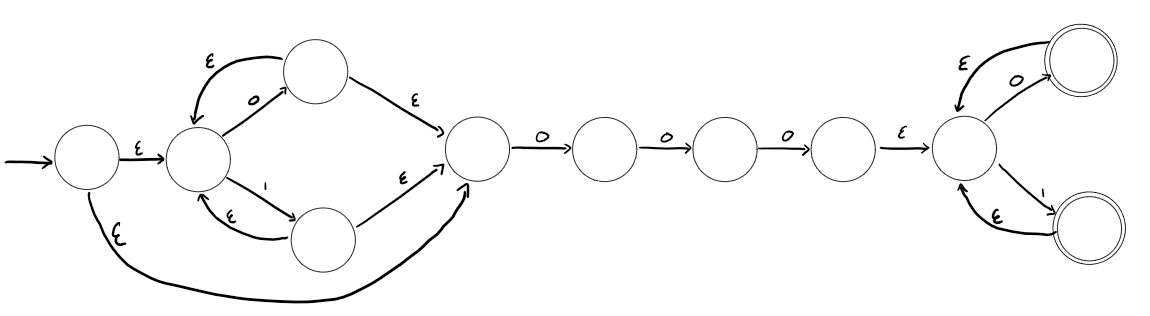
\includegraphics[width = 0.8\textwidth]{1_19a_CSCI338.PNG}
     \caption{Solution to 1.19.a}
     \label{fig:1.19.a}
 \end{figure}

\textbf{1.19.b}

\begin{figure}[H]
     \centering
     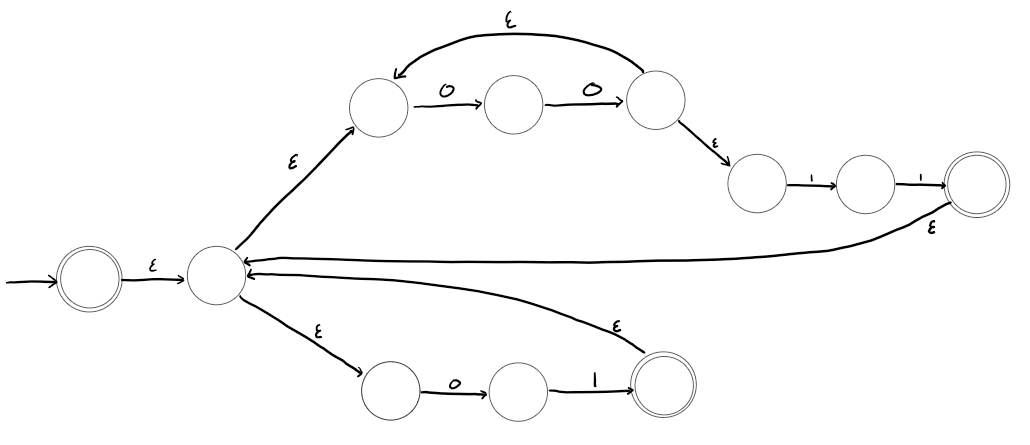
\includegraphics[width = 0.8\textwidth]{1_19b_CSCI338.PNG}
     \caption{Solution to 1.19.b}
     \label{fig:1.19.b}
 \end{figure}

\newpage
\section*{Problem 4}

Problem 1.21.a (page 86).
\newline

\textbf{1.21.a}

\begin{figure}[H]
     \centering
     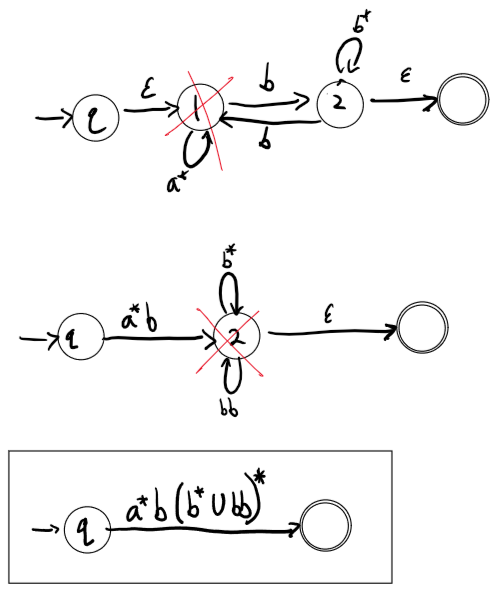
\includegraphics[width = 0.7\textwidth]{1_21a_CSCI338.PNG}
     \caption{Solution to 1.21.a}
     \label{fig:1.21.a}
 \end{figure}

\newpage
\section*{Problem 5}

Prove the following languages are not regular.
%blem 1.23.a, 1.23.c (page 88).

%(4.1) $A=\{www|w\in\{{\tt a,b}\}^*\}$.
(5.1) $A=\{a^{n^3}|n\geq 0\}$. Here $a^x$ means a string of $x$ $a$'s.
\newline

(5.2) $B=\{0^n1^m0^n|m,n\geq 0\}$.
\newline

\end{document}

